\documentclass[a4paper,chapter,atbegshi]{oblivoir}
\usepackage[dbl4x6]{fapapersize}
\usepackage{amsmath,amssymb,amsfonts,amsthm}
\usepackage{graphicx,xcolor,caption}
\usepackage{braket,hyperref,nicematrix}
\usepackage{euler,enumitem,tikz}
\usepackage{quantikz,wrapfig}
\usetikzlibrary{arrows.meta}
\setlist{nosep}
\hypersetup{
  colorlinks=true,linkcolor=teal,filecolor=magenta,urlcolor=cyan,
}
\title{\texttt{Introduction to Quantum Information Science} 학습일지}
\author{김태원}
\date{최초 작성 : 2023년 8월 29일 \\ 최근 편집 : \today}

\begin{document}
\maketitle
\break
\tableofcontents
\chapter{양자기초}
파인만{\tiny Richard Feynman}이 말하길 이중슬릿{\tiny double slit} 실험은
양자역학을 전부 요약한다. 

광자{\tiny photons}를 두 개의 슬릿{\tiny slit}을 지닌 벽에 하나씩 쏜다고 하자.
두 개의 슬릿 모두 개방될 때 광자가 특정 구간에 부딪히는 확률을 $P$, 1번 슬릿만
개방될 때 광자가 특정 구간에 부딪히는 확률을 $P_1$, 2번 슬릿만 개방될 때 광자가
특정 구간에 부딪히는 확률을 $P_2$라고 하자. 확률론에 따르면 당연히 $P=P_1+P_2$다.
그런데 실험 결과에 따르면 $P\neq P_1+P_2$다. 다시 말해 자연스러운 확률론은 자연의 
현상을 설명하지 못한다.

고전적인 확률론이 자연을 충분하게 설명하지 못하는데도 자연스러워 보이는 이유는 
\textbf{결어긋남\tiny decoherence}이라는 현상에서 비롯한다. 이를테면 상자를
열었을 때 슈뢰딩거의 고양이가 생과 사의 \emph{중첩\tiny superposition}으로
나타나지 않는다. 고양이가 제 환경과 끊임없이 상호작용하기 때문이다. 고양이와
환경 간의 상호작용은 고양이 계{\tiny system}의 정보를 누설한다. 반면 양자
중첩은 입자나 입자들의 군이 환경과 \emph{고립\tiny isolated}될 때 일어난다.

똑똑한 물리학자들이 이중슬릿 같은 실험을 통해 관찰한 바, 자연은 고전적인 확률
$P\in[0,1]$이 아니라 어떤 파동함수를 따른다. 그리고 이런 파동함수를 포착하는 
개념이 바로 \textbf{진폭\tiny amplitude} $\alpha\in\mathbb{C}$다. 양자역학에서
확률은 진폭을 사용해 \textbf{보른 규칙\tiny Born Rule}으로 정의된다. 보른 규칙은
보른{\tiny Max Born}이 양자계의 파동함수를 아우르는 슈뢰딩거 방정식의
해를 해석할 수 있는 유일한 방법으로 1926년에 제시한 공리다.
\begin{equation}\label{eq:11}
  P = |\alpha|^2 = \textrm{Real}(\alpha)^2+\textrm{Imaginary}(\alpha)^2
\end{equation}
진폭으로 이중슬릿 실험의 결과를 다시 확인하겠다. 두 슬릿 모두 개방될 때 광자가
특정 구간에 부딪히는 진폭을 $\alpha$, 1번 슬릿만 개방될 때 광자가 특정 구간에
부딪히는 진폭을 $\alpha_1$, 2번 슬릿만 개방될 때 광자가 특정 구간에
부딪히는 진폭을 $\alpha_2$라고 하자. 이떄 등식 $\alpha=\alpha_1+\alpha_2$는 모순을
유도하는가? $\alpha_1=a_1+b_1i, \alpha_2=a_2+b_2i$에 대해
\begin{align*}
  \alpha &= \alpha_1 + \alpha_2 \\
  \Rightarrow  P &= |\alpha|^2 \quad\quad\quad\quad[\textrm{보른 규칙}]\\ 
      &= |\alpha_1+\alpha_2|^2\\
      &= \textrm{Re}(\alpha_1+\alpha_2)^2+\textrm{Im}(\alpha_1+\alpha_2)^2\\
      &= (a_1+a_2)^2+(b_1+b_2)^2 \\
      &= (a_1^2+2a_1a_2+a_2^2)+(b_1^2+2b_1b_2+b_2^2) \\
      &= (a_1^2+b_1^2)+(a_2^2+b_2^2)+2(a_1a_2+b_1b_2)\\
      &= \textrm{Re}(\alpha_1)^2+\textrm{Im}(\alpha_1)^2+
      \textrm{Re}(\alpha_2)^2+\textrm{Im}(\alpha_2)^2+\overline{\alpha_1}\alpha_2+
      \alpha_1\overline{\alpha_2}\\
      &=|\alpha_1|^2+|\alpha_2|^2+\overline{\alpha_1}\alpha_2+
          \alpha_1\overline{\alpha_2} 
\end{align*}
이때 진폭이 복소수로 정의되기에 $\alpha$가 음수일 수 있으므로 모순이 유도되지
않는다는 사실을 아래처럼 나타낼 수 있다.
\[
  \alpha_1 := \frac{1}{2}, \alpha_2 := -\frac{1}{2} \Rightarrow
  \begin{cases}
    |\alpha_1|^2 = \frac{1}{4}, |\alpha_2|^2=\frac{1}{4} \\
              |\alpha=\alpha_1+\alpha_2|^2=0
  \end{cases}
\]
이처럼 두 상태의 진폭이 서로 소거할 수도 있다. \textbf{간섭\tiny
interference}이라는 현상이다. 간섭은 간단한 선형대수학으로 설명될 수 있다.
우선 2-노름{\tiny norm} $\alpha^2+\beta^2=1$을 충족하는 벡터 $(\alpha,\beta)$가
아래와 같은 원을 형성한다는 사실에 주목한다. 
\begin{figure}[h]
\begin{center}
  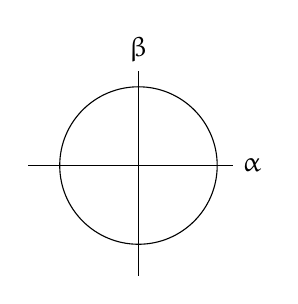
\begin{tikzpicture}
    \draw[fill=none](0,0)circle(1.0); 
    \draw[](0,-1.4)--(0,1.2) node[above]{$\beta$};
    \draw[](-1.4,0)--(1.2,0) node[right]{$\alpha$};
  \end{tikzpicture}
  \caption{유클리드 노름\label{fig:1-1}}
\end{center}
\end{figure}
2-노름을 유클리드 노름{\tiny Euclidean norm}이라고 부르기도 한다.
임의의 $\alpha,\beta$에 대해 위와 같은 원이 형성되기에 한 유클리드 노름 단위
벡터를 다른 유클리드 노름 단위 벡터로 사상하는{\tiny maps to} 행렬 혹은 변환이
존재할 수 있다. 이를 \textbf{유니타리 행렬\tiny unitary matrix}이라고 부른다.
또한 여기서 `유클리드 노름 단위 벡터'가 바로 \textbf{큐비트\tiny qubit}다. 

물리학자들은 디락{\tiny Paul Dirac}이 도입한 브라-켓{\tiny bra-ket} 표기법으로
큐비트를 나타낸다. 켓{\tiny ket} $\ket{\psi}$과 브라{\tiny bra} $\bra{\psi}$는
아래와 같다.
 \[
   \ket{\psi} = \alpha\ket0+\beta\ket1 = \begin{pmatrix}\alpha\\\beta\end{pmatrix}
  =\alpha\begin{pmatrix}1\\0\end{pmatrix}+\beta\begin{pmatrix}0\\1\end{pmatrix},
  \quad
  \bra{\psi} = \overline{\alpha}\bra0 +\overline{\beta}\bra1=
   \begin{pmatrix}\overline{\alpha}&\overline{\beta}\end{pmatrix}
 \]
이에 유클리드 노름 $\|\psi\|^2$가 자연스럽게 정의될 수 있다. 
 \[
   \|\psi\|^2 = \begin{pmatrix}\overline{\alpha}&\overline{\beta}\end{pmatrix}
   \begin{pmatrix}\alpha\\\beta\end{pmatrix}=|\alpha|^2+|\beta|^2
 \]
 내적 $\braket{\psi|\phi}$는 아래 성질을 만족한다.
 \begin{align*}
   \braket{\psi|\phi} &= 
   \begin{pmatrix}\overline{\alpha_1} &\overline{\beta_1}\end{pmatrix}
   \begin{pmatrix}\alpha_2\\\beta_2\end{pmatrix} \\
    &= \overline{\alpha_1}\alpha_2+\overline{\beta_1}\beta_2\\
    &=\overline{\alpha_1}\overline{\overline{\alpha_2}}+
    \overline{\beta_1}\overline{\overline{\beta_2}} \\
    &= \begin{pmatrix}\overline{\overline{\alpha_2}} & \overline{\overline{\beta_2}}\end{pmatrix}
   \begin{pmatrix}\overline{\alpha_1}\\\overline{\beta_2}\end{pmatrix}
   = \overline{\braket{\phi|\psi}}
 \end{align*}
 여기서 $\alpha$는 $\ket{0}$이라는 결과에 대한 진폭이고 $\beta$는 $\ket{1}$이라는
결과에 대한 진폭이다. 따라서 상태 $\ket\psi$에서 상태 $\ket\phi$에 이르는
확률 $P(\ket\phi)$의 보른 규칙을 아래처럼 다시 쓸 수 있다.
\[
  P(\ket\phi)=|\braket{\psi|phi}|^2
\]
이에 행렬을 $45^{\circ}$ 즉 $\frac{\pi}{4}$만큼 회전하며 노름을 보존하는
아래 같은 유니타리 행렬이 있다.
\[
  \begin{pmatrix}
    \cos\frac{\pi}{4} &-\sin\frac{\pi}{4}\\
    \sin\frac{\pi}{4} &\cos\frac{\pi}{4}
  \end{pmatrix}
  = \begin{pmatrix}
    \frac{1}{\sqrt{2}} &-\frac{1}{\sqrt{2}} \\
    \frac{1}{\sqrt{2}} &\frac{1}{\sqrt2}
  \end{pmatrix}
\]
$\ket0$를 위 유니타리 행렬로 변환한다.
\begin{equation}\label{eq:1-2}
  \begin{pmatrix}
    \frac{1}{\sqrt{2}} &-\frac{1}{\sqrt{2}} \\
    \frac{1}{\sqrt{2}} &\frac{1}{\sqrt2}
  \end{pmatrix}
  \begin{pmatrix}
    1\\0
  \end{pmatrix}
  =\begin{pmatrix}
    \frac{1}{\sqrt2}\\\frac{1}{\sqrt2}
  \end{pmatrix}
\end{equation}
$\frac{1}{\sqrt2}\ket{0}+\frac{1}{\sqrt2}\ket{1}$을 다시 위 유니타리 행렬로
변환한다.
\[
  \begin{pmatrix}
    \frac{1}{\sqrt{2}} &-\frac{1}{\sqrt{2}} \\
    \frac{1}{\sqrt{2}} &\frac{1}{\sqrt2}
  \end{pmatrix}
  \begin{pmatrix}
    \frac{1}{\sqrt2}\\\frac{1}{\sqrt2}
  \end{pmatrix}
  =\begin{pmatrix}0\\1\end{pmatrix}=\ket{1}
\]
즉 무작위 상태 $\frac{1}{\sqrt2}\ket{0}+\frac{1}{\sqrt2}\ket{1}$에 위 유니타리
행렬과 같은 무작위 연산을 적용하면 $\ket{1}$이라는 결과가 결정론적{\tiny
deterministic}으로 나온다. 여기 무작위 연산을 다시 적용하여 나타난 무작위 상태
 $-\frac{1}{\sqrt2}\ket{0}+\frac{1}{\sqrt2}\ket{1}$에 무작위 연산을 또다시
 적용하면 $\ket{0}$이라는 결과가 결정론적으로 나온다. 이것이 앞서 언급한
 \textbf{간섭} 개념의 선형대수학적 바탕이다. 

 위 유니타리 행렬에 대해 $\ket{0}$이라는 결과를 결정론적으로 도출하는 행렬은
 $\frac{1}{\sqrt2}\ket0-\frac{1}{\sqrt2}\ket{1}$이다. 이를 \textbf{경로\tiny
 path}가 두 개 존재하여 한 경로는 음의 진폭 $-\frac{1}{\sqrt2}$를 지니고 
 다른 경로는 양의 진폭 $\frac{1}{\sqrt2}$을 지닌다고 표현한다. 그리고 이 경우
 두 경로는 \textbf{파괴적 간섭\tiny destructive interference} 관계에 놓인다. 
 반면 $\ket{1}$이라는 결과를 결정론적으로 도출하는 경로는 모두 양의 진폭
 $\frac{1}{\sqrt2}$을 지녀 \textbf{구성적 간섭\tiny constructive interference}
 관계다.

 이제 그림 \ref{fig:1-1}상의 원을 다시 그린다.
\begin{figure}[h]
\begin{center}
  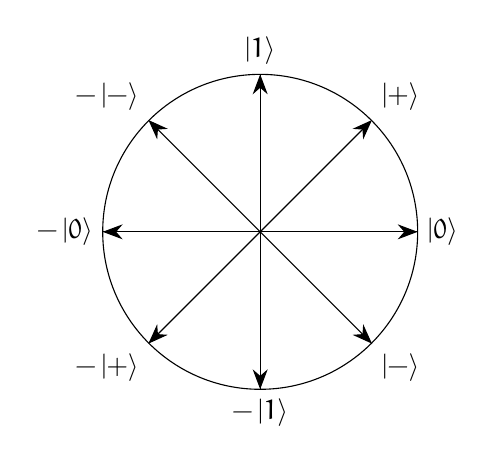
\begin{tikzpicture}
    \draw[fill=none](0,0)circle(2.0);
    \draw[-{Stealth[scale=1.5]}] (0,0)--(0,2);
    \draw[-{Stealth[scale=1.5]}] (0,0)--(-2,0) node[left]{$-\ket0$};
    \draw[-{Stealth[scale=1.5]}] (0,0)--(1.42,1.42) node[above right]{$\ket+$};
    \draw[-{Stealth[scale=1.5]}] (0,0)--(2,0);
    \draw[-{Stealth[scale=1.5]}] (0,0)--(-1.42,1.42) node[above left]{$-\ket-$};
    \draw[-{Stealth[scale=1.5]}] (0,0)--(1.42,-1.42) node[below right]{$\ket-$};
    \draw[-{Stealth[scale=1.5]}] (0,0)--(0,-2) node[below]{$-\ket1$};
    \draw[-{Stealth[scale=1.5]}] (0,0)--(-1.42,-1.42) node[below left]{$-\ket+$};
    \draw[](0,-2.0)--(0,2.0) node[above]{$\ket1$};
    \draw[](-2.0,0)--(2.0,0) node[right]{$\ket0$};
  \end{tikzpicture}
  \caption{직교 행렬\label{fig:1-2}}
\end{center}
\end{figure}
여기서 $\{\ket+,\ket-\}$는 \emph{아다마르 기저\tiny Hadamard basis}라는 것인데
앞서 예로 든 $45^{\circ}$ 회전 유니타리 변환 과정 \ref{eq:1-2}에서 이미
확인한 적 있다. 
\[
  \begin{pmatrix}\frac{1}{\sqrt2}\\\frac{1}{\sqrt2}\end{pmatrix}=\ket+ =
  \frac{\ket0+\ket1}{\sqrt2},\quad\begin{pmatrix}\frac{1}{\sqrt2}\\
  -\frac{1}{\sqrt2}\end{pmatrix} = \ket-=\frac{\ket0-\ket1}{\sqrt2}
\]
아다마르 기저는 \textbf{아다마르 게이트}{\tiny gate}\footnote{양자정보론에서는
작은 유니타리 변환을 게이트라고 부른다.} $H:\{\ket0,\ket1\} \rightarrow
\{\ket+,\ket-\}$ 를 형성한다. 이를테면 $\ket0$에 $H$를 적용한 결과는 아래와 같다.
\[
  H\ket0=\frac{1}{\sqrt2}\begin{pmatrix}1&1\\1&-1\end{pmatrix}
  \begin{pmatrix}1\\0\end{pmatrix} =
  \begin{pmatrix}\frac{1}{\sqrt2}\\\frac{1}{\sqrt2}\end{pmatrix}=\ket+
\]
그림 \ref{fig:1-2}에서 확인할 수 있는 사실은 $\frac{\pi}{4}$
회전과 반사만으로 여덟 가지 상태를 나타낼 수 있다는 것과 원의 방정식에 의해
유니타리 변환이 유클리드 노름을 보존한다는 것이다. 가령 임의의 유니타리 행렬
$U$의 복소전치행렬 $U^{\dagger}$를 $U$로 변환하면 항등행렬 $I$가 나온다.
\[
  \braket{\psi|\psi} = (\ket{\psi})^{\dagger}\ket{\psi} 
              = (U\ket{\psi})^{\dagger}U\ket{\psi}
              =\braket{\psi|U^{\dagger}U|\psi} 
  \iff\forall\ket{\psi},U^{\dagger}U= I
\]
유니타리 변환은 선형변환이기도 해서 $U(c\ket0)=cU\ket0$이 임의의 상수 $c$에 
대해 성립할 수 있다. 여기서 $c$가 어떤 $\theta$에 대해 오일러 공식 
$e^{i\theta}=\cos\theta+i\sin\theta$\footnote{오일러 공식은 슈뢰딩거
방정식을 비롯해 양자역학에서 중요한 파동-삼각함수를 지수함수로 변환할 수 있도록
하는, 복소평면에서 일정한 속도로 원운동하는 물체의 위치 방정식이다.}를 만족하면 
\textbf{전역위상\tiny global phase}이라고 한다. 다만 $\ket{\psi}$와 
$e^{i\theta}\ket{\psi}$가 물리적으로 구분될 수 없기에 전역위상은
관찰불가능하다. 전역위상이 관찰가능하다는 말은 큐비트와 같은
양자계에 어떤 스칼라를 곱해서 우주 전체를 살짝 옮길 수 있다는
소리와 같다. 이에 반해 관찰 가능한 것은 바로 \textbf{상대위상\tiny relative
phase}이다. 가령 $\ket+$와 $\ket-$라는 두 상태 간에는 상대위상차이가 관측될 수
있는데, $\ket-$에서 $\ket+$에 이르는 일련의 유니타리 연산들이 존재하기 때문이다.

관찰 혹은 측정{\tiny measurment}과 가능한 유니타리 연산들에는 차이가 존재하는
셈이다. 유니타리 변환이 (그 복소전치행렬로 인해) 가역{\tiny invertible}이고
결정론적이며 (복소수 행렬이기에 모든 $a$에 대해 $\sqrt{a}$를 내놓을 수 있어서)
연속적인 반면, 측정은 비가역{\tiny irreversible}이고 확률론적, 비연속적이다.
이처럼 판이한 유니타리 변환과 측정을 이어주는 것이 바로 유클리드 노름이다.
유니타리 변환은 유클리드 노름을 보존하고 측정은
유클리드 노름으로 결정되는 확률을 제공한다. 그리고 이에 따른 연속과 비연속,
결정론과 확률론의 상호작용을 극단적으로 소진하는 사고실험이 바로 \emph{튜링의
역설} 혹은 \textbf{양자 제논 효과}다.

$\ket0$이나 $\ket1$로 설정된 큐비트가 있다고 하겠다. 이 큐비트에 유니타리
변환을 전혀 사용하지 않으면서 상태를 바꿀 수 있을까? 아주 작은 $\epsilon$에 
대해 $\{\ket0,\ket1\}$에서 $\epsilon$만큼 회전한 기저는 아래처럼 측정할 수 있다.
\begin{align*}
  \begin{aligned}
  \ket0\mapsto\ket{v}&= \cos\epsilon\ket0+\sin\epsilon\ket1\\
  \Rightarrow 
    P(\ket{v})&=|\braket{0|v}|^2 \\
              &=\left|\begin{pmatrix}1,0\end{pmatrix}
              \begin{pmatrix}\cos\epsilon\\\sin\epsilon\end{pmatrix}\right|^2 \\
              &=|\cos\epsilon|^2 \approx{\biggl(1-\frac{\epsilon^2}{2}\biggr)^2}\\
              &= 1-\epsilon^2+\frac{\epsilon^4}{4}
              \approx 1-\epsilon^2 \\
  \end{aligned}
  \begin{aligned}
  \ket1\mapsto\ket{w}&=-\sin\epsilon\ket0+\cos\epsilon\ket1\\
    P(\ket w)&=|\braket{1|w}|^2 \\
              &=\left|\begin{pmatrix}0,1\end{pmatrix}
              \begin{pmatrix}-\sin\epsilon\\\cos\epsilon\end{pmatrix}\right|\\
              &=|\cos\epsilon|^2 \approx \biggl(1-\frac{\epsilon^2}{2}\biggr)^2\\
              &= 1-\epsilon^2+\frac{\epsilon^4}{4}
              \approx1-\epsilon^2
  \end{aligned}
\end{align*}
큐비트가 $\epsilon$만큼 회전할 수 있는 확률은 $\epsilon$이 감소할수록 
증가\footnote{근사값의 유도에 관해서는 \href{https://en.wikipedia.org/wiki/Small-angle_approximation}{작은 각도 근사}를 참고하라.}한다.
그러니 이 절차를 대략 $\frac{1}{\epsilon}$번 반복하며 매번 $\epsilon$만큼 
회전하면, $\ket0$을 아주 천천히 $\ket1$로 옮길 수 있다. 이 과정이
성공하지 \emph{않을} 확률은 $1-(1-\epsilon^2)=\epsilon^2$에 $\frac{1}{\epsilon}$을
곱한 $\epsilon$이다. 그리고 $\epsilon$은 가정에 의해 극미량이다.
따라서 유니타리 변환이 없어도 아주 높은 확률로 상태를 바꿀 수 있다. 

그런데 이게 무슨 소리인가? 비유하자면, 홍길동의
$\ket{\textrm{미혼}}$ 상태를 $\ket{\textrm{기혼}}$ 상태로 바꾸는
유니타리 변환 수준의 깔끔한 방법은 당장 김철수와 서류상
혼인신고하는 것이다. 이 방법은 지금 어렵다고 할 때,
적어도 홍길동이 김철수를 1년간 그냥 지켜보다가 어느 날 갑자기 프로포즈하는
쪽보다는 홍길동이 1년을 $\frac{1}{\epsilon}$ 정도로 아주 잘게 나눠 $\epsilon$
만큼의 애정 표현을 반복하는 쪽이 결혼 확률이 더 높을 것이다.

다음 예는 \textbf{엘리추르-바이드만 폭탄\tiny Elitzur-Vaidman Bomb}이다.
양자 공항이 배경이다. 화물 하나에 폭탄이 존재하는 것 같은데, 폭탄이 있다면
화물을 여는 순간 폭발할 것이 분명하다. 폭탄이 폭발할 확률을 최소화할 수 있을까?

우선 $\ket0$을 초기 상태로 둔다. 화물 확인이라는 행동은 회전 
$R_{\epsilon}$으로 정의한다. 
\[
  R_{\epsilon} = \begin{pmatrix}\cos\epsilon&-\sin\epsilon\\
  \sin\epsilon &\cos\epsilon\end{pmatrix}
\]
폭탄이 없다면, 그대로 $\cos\epsilon\ket0+\sin\epsilon\ket1$이다. 폭탄이 있다면,
폭탄은 $\{\ket0,\ket1\}$을 기저로 측정된다. 다시 말해 회전-확인의 결과가
$\ket0$이라면 폭탄이 폭발하지 않은 것이다. 그리고 결과가 $\ket1$이라면
폭탄이 폭발한 것이다. 

초기 상태 $\ket0$에 대해 화물을 한 번 확인-$R_{\epsilon}$한 결과는
$\cos\epsilon\ket0+\sin\epsilon\ket1$이다. 폭탄이 존재할 때,
 폭탄이 폭발할 확률 $P(1)$은 $\cos\theta\ket0+\sin\epsilon\ket1$이
$\ket1$로 관측될 확률과 같다. 
\begin{align*}
  P(1) &= |\braket{b|1}|^2 \\
       &= \left|\begin{pmatrix}\cos\epsilon &\sin\epsilon\end{pmatrix}
       \begin{pmatrix}0\\1\end{pmatrix}\right|^2\\
       &=|\sin\epsilon|^2 \approx \epsilon^2
\end{align*}
따라서 이 과정을 대략 $\frac{\pi}{2\epsilon}$번\footnote{여기서 
$\frac{\pi}{2\epsilon}$은 $90^{\circ}$보다 아주 약간 작은 각도로, 그림 
\ref{fig:1-2}의 원에서 `$\ket1$' 직전에 해당한다.} 
반복하며 매번 $R_{\epsilon}$을 적용하면, 존재하는 폭탄이 터지는 확률은
$\frac{\pi}{2\epsilon}\epsilon^2 =\frac{\pi}{2}\epsilon$에 불과하다. 따라서
양자 공항에서는 대단히 높은 확률로 폭탄이 폭발하지 않는다.

\section*{부록; 양자회로}
그림 \ref{fig:1-3}은 $\ket1$로 초기 상태를 설정한 다음 두 아다마르 게이트를
적용하여 표준기저 $\{\ket0,\cdots,\ket{N-1}\}$상의 측정으로 종결하는 
양자회로\footnote{논리회로를 배울 때처럼 양자 게이트도 언젠간 다 외워야
한다. \href{https://en.wikipedia.org/wiki/Quantum_logic_gate}{위키피디아}를
참고하라.}다. 양자회로는 여러 큐비트에 대한 연산을 표기할 수도 있다. 
그림 \ref{fig:1-4}는 이중 큐비트 게이트 $U$에 대해 첫 번째 큐비트로 
아다마르 게이트를 적용한 다음 두 큐비트를 모두 측정하는 양자회로다.
\begin{figure}[h]
\begin{minipage}{0.48\textwidth}
\centering
\begin{quantikz}
  \lstick{$\ket1$}&\gate{H}&\gate{H}&\meter{} 
\end{quantikz}
\caption{양자 회로 예제\label{fig:1-3}}
\end{minipage}\hfill
\begin{minipage}{0.48\textwidth}
\centering
  \begin{quantikz}
    \lstick{$\ket0$}&\gate[2]{U}&\gate{H}&\meter{} \\
    \lstick{$\ket0$}& &\qw &\meter{} 
  \end{quantikz}
  \caption{이중 양자 회로 예제\label{fig:1-4}}
\end{minipage}
\end{figure}

\noindent
그림 \ref{fig:1-5} 좌측의 양자회로는 제어{\tiny controlled} 게이트를 사용한다. 
첫 줄에 놓인 $\bullet-\oplus$는 제어 NOT 혹은 CNOT 게이트를 나타내고 이는
첫 비트 혹은 제어 큐비트가 $\ket1$이면 두 번째 큐비트를 반전{\tiny flip}한다. 그 다음 줄에 놓인 $\bullet- U$는 임의의 $U$에 대해 제어 $U$ 게이트를 
나타내며 제어 큐비트가 $\ket1$이면 $U$를 적용한다.
\begin{figure}[h]\centering
  \begin{quantikz}
    & \ctrl{1} & \ctrl{1} & \targ{} & \qw \\
    & \targ{} & \gate{U} & \ctrl{-1} & \qw
  \end{quantikz}
  여기서
  \begin{quantikz}
    &\targ{}&\qw \\
    &\ctrl{-1}&\qw
  \end{quantikz}
  =\begin{quantikz}
    &\gate{H}&\ctrl{1}&\gate{h}&\qw\\
    &\gate{H}&\targ{}&\gate{h}&\qw
  \end{quantikz}
  \caption{제어 양자 회로 예제\label{fig:1-5}}
\end{figure}
마지막 줄은 우측 도면과 같다.
\chapter{양자얽힘}
두 큐비트의 상태는 아래와 같다. 
\[
  \ket{\psi} = \alpha\ket{00}+\beta\ket{01}+\gamma\ket{10}+\delta\ket{11}
\]
네 가지 결과는 보른 규칙 \ref{eq:11}에 의해 아래 같은 확률을 지닌다. 
\[\begin{matrix}
  P(\ket{00})=|\alpha|^2 & P(\ket{01})=|\beta|^2 \\
  P(\ket{10})=|\gamma|^2 & P(\ket{11})=|\delta|^2
\end{matrix}\]
첫 번째 큐비트가 $\ket{0}$이라는 정보가 주어질 때 두 번째 큐비트는 아래
같은 중첩으로 주어질 수 있다.
\begin{equation}\label{eq:2-1}
  \ket0\otimes\frac{\alpha\ket0+\beta\ket1}{\sqrt{|\alpha|^2+|\beta|^2}}
  = \begin{bmatrix}1\\0\end{bmatrix}\otimes
  \begin{bmatrix}\alpha\\\beta\end{bmatrix}\frac{1}{\sqrt{|\alpha|^2+|\beta|^2}}
  = \begin{bmatrix}\alpha\\\beta\\0\\0\end{bmatrix}\frac{1}{\sqrt{|\alpha|^2+|\beta|^2}}
\end{equation}
여기서 $\sqrt{|\alpha|^2+|\beta|^2}$로 나누는 걸 정규화{\tiny normalization}라고
부른다. \emph{노름}화라고 이해할 수도 있는데 왜냐하면 $\alpha$와 $\beta$ 서로만
있어도 유클리드 노름의 조건을 유지하도록 보조하는 연산이기 때문이다. 
\[
  \Bigg\lvert\frac{\alpha}{\sqrt{|\alpha|^2+|\beta|^2}}\Bigg\rvert^2 +
  \Bigg\lvert\frac{\beta}{\sqrt{|\alpha|^2+|\beta|^2}}\Bigg\rvert^2
  =
  \frac{|\alpha|^2+|\beta|^2}{|\alpha|^2+|\beta|^2}=1
\]
중첩 \ref{eq:2-1}를 \textbf{부분측정규칙\tiny partial measurement rule}이라고
부르는 양자역학의 기본 규칙이다. 1장에서 다룬 양자역학 기초와 부분측정규칙만으로
학부 수준 양자정보학은 전부 유도할 수 있다. 2장은 부분측정규칙을 풍성하게
이해하기 위해 1장에서 다룬 내용을 돌이킨다. 

아래 게이트는 첫 큐비트에 아무것도 하지 않고 두 번째 큐비트에 NOT 게이트를
적용\footnote{가령 $\ket{a0}$에 대해 $\ket{a}$는 가만히 놔두고 두 번째 
큐비트만 반전하여 $\ket{a1}$을 출력하는 식이다. 또한 행렬 주변의
첨자 $00, 01, 10, 11$은 행에서 입력을 나타내고 열에서 출력을 나타낸다.
가령 CNOT 게이트는 $11$이라는 입력에 대해 $10$을 출력한다.}한다. 
\[
  \begin{bNiceMatrix}[first-col, first-row]
    & \scriptstyle00 & \scriptstyle01 & \scriptstyle10 & \scriptstyle11 \\
    \scriptstyle00 & 0 & 1 & 0 & 0 \\
    \scriptstyle01 & 1 & 0 & 0 & 0 \\
    \scriptstyle10 & 0 & 0 & 0 & 1 \\
    \scriptstyle11 & 0 & 0 & 1 & 0
  \end{bNiceMatrix}
\]
이 게이트를 텐서곱{\tiny tensor product}으로 나타낼 수도 있다.
\[
  I\otimes \textrm{NOT} = \begin{bmatrix}1 & 0 \\ 0 & 1\end{bmatrix}
  \otimes \begin{bmatrix}0 & 1 \\ 1 & 0\end{bmatrix}
\]
감으로 텐서곱이 어떤 연산인지 파악하길 바란다. 요는 ``두 번째 큐비트에 NOT
게이트를 적용''과 같은 표현의 뜻이다. 첫 번째 큐비트에 아다마르 게이트를
적용하고 두 번째 큐비트에 다시 아다마르 게이트를 적용한다는 말은 텐서곱으로
$H\otimes H$와 같으며 게이트로는 아래와 같다.
\[
  \frac{1}{\sqrt2}\begin{bmatrix}1&1\\1&-1\end{bmatrix}\otimes
  \frac{1}{\sqrt{2}}\begin{bmatrix}1&1\\1&-1\end{bmatrix}=\frac{1}{2}
  \begin{bNiceMatrix}[first-col, first-row]
    & \scriptstyle00 & \scriptstyle01 & \scriptstyle10 & \scriptstyle11 \\
    \scriptstyle00 & 1 & 1 & 1 & 1 \\
    \scriptstyle01 & 1 & -1 & 1 & -1 \\
    \scriptstyle10 & 1 & 1 & -1 & -1 \\
    \scriptstyle11 & 1 & -1 & -1 & 1
  \end{bNiceMatrix}
\]
여기서 $00$이라는 첨자를 지니는 첫 번째 행이 구성되는 방식을 $H\otimes H\ket{00}=
\ket{++}$이라는 텐서곱으로 생각할 수 있다. 마찬가지로 $01$이라는 첨자를 지니는
두 번째 행이 구성되는 방식을 $H\otimes H\ket{01}=\ket{+-}$이라는 텐서곱으로
받아들일 수 있다.
\[
  \ket{+-}=\ket{+}\otimes\ket{-}=
  \frac{\ket0+\ket1}{\sqrt{2}}\otimes\frac{\ket0-\ket1}{\sqrt2}=
  \begin{bmatrix}\frac{1}{\sqrt{2}}\\\frac{1}{\sqrt2}\end{bmatrix}\otimes
  \begin{bmatrix}\frac{1}{\sqrt2}\\-\frac{1}{\sqrt2}\end{bmatrix} =
  \begin{bmatrix}\frac{1}{2}\\-\frac{1}{2}\\\frac{1}{2}\\-\frac{1}{2}\end{bmatrix}
  = \frac{1}{2}\begin{bNiceMatrix}[first-row] 
  \scriptstyle01\\1\\-1\\1\\-1\end{bNiceMatrix}
\]
지금껏 2-큐비트 유니터리를 1-큐비트 유니터리의 텐서곱으로 구성할 수 있었다.
다만 CNOT 게이트는 이게 안 된다. 첫 번째 큐비트가 $0$이면 두 번째 큐비트를 놔두고
첫 번째 큐비트가 $1$이면 두 번째 큐비트를 반전하는 CNOT 게이트는 아래처럼 생겼다.
\[
  \begin{bNiceMatrix}[first-col, first-row]
    & \scriptstyle00 & \scriptstyle01 & \scriptstyle10 & \scriptstyle11 \\
    \scriptstyle00 & 1 & 0 & 0 & 0 \\
    \scriptstyle01 & 0 & 1 & 0 & 0 \\
    \scriptstyle10 & 0 & 0 & 0 & 1 \\
    \scriptstyle11 & 0 & 0 & 1 & 0
  \end{bNiceMatrix}
\]
다시 말해 CNOT은 한 큐비트가 다른 큐비트한테 영향을 미치는 게이트다. CNOT의
이런 성질을 사용해 특이한 상태를 만들어낼 수 있다. 아래는 \textbf{벨 쌍\tiny
Bell Pair} 혹은 \textbf{EPR 쌍}, \textbf{싱글렛\tiny singlet}이라고 부르는
쌍이다. 
\[
  (CNOT)(H\otimes I)\begin{bmatrix}1\\0\\0\\0\end{bmatrix}
  \longrightarrow 
  CNOT\begin{bmatrix}\frac{1}{\sqrt2}\\0\\\frac{1}{\sqrt2}\\0\end{bmatrix}
  \longrightarrow
  \begin{bmatrix}\frac{1}{\sqrt{2}}\\0\\0\\\frac{1}{\sqrt2}\end{bmatrix}
\]
CNOT의 첫 큐비트와 두 번째 큐비트를 텐서곱으로 분해할 수 없으므로 벨 쌍
또한 첫 큐비트와 두 번째 큐비트의 상태가 텐서곱으로 분해되지 않는다. 이런 
상태를 \textbf{얽힘\tiny entanglement} 혹은 \emph{순수 상태}라고 부른다. EPR 쌍은
이름만 무려 세 개인 만큼 중요한 상태이기 때문에 회로와 브라켓도 기억해둔다.

\begin{figure}[h]
  \centering
  \begin{minipage}{0.3\textwidth}
  \begin{quantikz}
  \lstick{$\ket0$}&\gate{H}&\ctrl{1}&\qw\\
  \lstick{$\ket0$}&\qw&\targ{}&\qw
  \end{quantikz}
\end{minipage}
\begin{minipage}{0.5\textwidth}
\[
  \ket{00}\longrightarrow\ket+\otimes\ket0=\frac{\ket{00}+\ket{10}}{\sqrt2}
  \longrightarrow\frac{\ket{00}+\ket{11}}{\sqrt2}
\]
\end{minipage}
\caption{EPR 쌍}
\end{figure}

얽힘은 양자역학을 구성하는 수학의 필연적인 귀결이다. 또한 얽힘은 (EPR 쌍에서 `E'에
해당하는) 아인슈타인이 양자역학에 신경질을 부린 이유다. 
달에는 철수가 있고 지구에는 영희가 있다고 하겠다. 철수와 영희는 입자의 쌍에
얽힘을 부여할 수 있다. EPR 쌍, 즉 $\frac{\ket{00}+\ket{11}}{\sqrt2}$로 상태를
설정하는 것이다. 그리고 철수가 입자를 측정하는 \underline{바로 그때} 철수는 영희가
관측할 상태가 $\ket{0}$인지 $\ket{1}$인지 알 수 있다. 

여타 물리학자와 다르게 아인슈타인에게는 이 사실이 아주 거슬렸다. 1935년,
아인슈타인, 포돌스키{\tiny Podolsky}, 로젠{\tiny Rosen}은
이 문제를 확대하는 논문을 발표한다. 철수가 $\{\ket0,\ket1\}$이 아니라 $\{\ket+,
\ket1\}$을 기저로 측정하면 어떻게 되는가? 

이 물음은 철수가 자신의 큐비트에 아다마르 게이트를 적용한 다음 $\{\ket0,\ket1\}$을
기저로 측정하는 상황을 통해 나타낼 수 있다.
\begin{align*}
  (H\otimes I)\left(\frac{\ket{00}+\ket{11}}{\sqrt2}\right)
  =\;&
  \frac{\ket{00}+\ket{01}+\ket{10}-\ket{11}}{2} 
\end{align*}
부분측정규칙 \ref{eq:2-1}을 적용한다. 철수가 $\ket0$을 보면 영희의 큐비트는
아래처럼 붕괴하고\footnote{여기서 $\frac{1}{\sqrt2}$는 
$\sqrt{\left(\frac{1}{2}\right)^2+\left(\frac{1}{2}\right)^2}$로 정규화하는
값이다.}
\[
  \frac{\ket0+\ket1}{\sqrt2}=\ket+
\]
철수가 $\ket1$을 보면 영희의 큐비트는 아래처럼 붕괴한다.
\[
  \frac{\ket0-\ket1}{\sqrt2}=\ket-
\]
아인슈타인, 포돌스키, 로젠은 이게 왜 거슬렸는가? 철수가 $\{\ket0,
\ket1\}$을 기저로 EPR 상태를 측정하면 영희가 $\ket0$이나 $\ket1$을 보고, 철수가
$\{\ket+,\ket-\}$를 기저로 측정하면 영희가 $\ket+$이나 $\ket-$을 보는데, 이런
의사소통{\tiny communication}이 \underline{즉각적으로} 혹은 \underline{바로 그때}
이루어진다는 사실이다. 따라서 빛보다 빠른 의사소통이 존재하며, 이는 얽힘이라는
양자역학적 현상이 상대성이론의 근본 규칙에 대해 모순을 유도한다는 뜻이다.

다행히 이들을 화해시키는 방법이 존재한다. 순수상태 뿐만 아니라 
\textbf{혼합상태\tiny mixed states}도 논의에 끌어들이는 방법이다. 혼합상태란
양자 상태 $\ket{\psi}$에 대한 확률 $p_i$의 분포 $\{p_i,\ket{\psi_i\}}$이다.
그리고 화해의 핵심은 바로 상이한 확률분포를 지니는 순수상태들이 정확히
서로 같은 혼합상태로 나타낼 수 있다는 사실에 달렸다. 

우선 어느 양자계에 관한 모든 물리적으로 관찰가능한 정보를 고유하게 나타낼 수
있도록 하는 \textbf{밀도행렬\tiny density matrix}을 살핀다. 혼합상태 
$\{p_i,\ket{\psi}\}$에 대한 밀도행렬 표현은 아래처럼 주어진다. 
\begin{equation}
  \rho = \sum_i p_i\ket{\psi_i}\bra{\psi_i}
\end{equation}
여기서 $\ket{\psi_i}\bra{\psi_i}$는 \textbf{외적}을 나타낸다.
\[
  \begin{bmatrix}\alpha_0\\\alpha_1\\\vdots\\\alpha_{N-1}\end{bmatrix}
  \begin{bmatrix}\overline{\alpha_0} & \overline{\alpha_1} &\cdots 
  &\overline{\alpha_{N-1}}\end{bmatrix} = \begin{bmatrix}
    |\alpha_0|^2 & & &  \\
    & \ddots & \alpha_i\overline{\alpha_j}& \\
    &\alpha_j\overline{\alpha_i}&\ddots&\\
    &&&|\alpha_{N-1}|^2
  \end{bmatrix}
\]
보시다시피 혼합상태의 밀도행렬 $\rho$는 $\rho$ 자신과 켤레 전치 $\rho^{\dagger}$가
같은 \emph{에르미트 행렬\tiny Hermitian matrix}이다. 표준 기저에 
대한 외적은 아래와 같다.
\[
  \ket0\bra0=\begin{bmatrix}1&0\\0&0\end{bmatrix},\quad
  \ket1\bra1=\begin{bmatrix}0&0\\0&1\end{bmatrix}
\]
이들을 균등하게 섞으면 아래와 같다.
\[
  \frac{\ket0\bra0+\ket1\bra1}{2} =
  \begin{bmatrix}\frac{1}{2}&0\\0&\frac{1}{2}\end{bmatrix}
  =\frac{I}{2}
\]
$\{\ket+,\ket-\}$에 대해서는 아래와 같다.
\[
  \ket+\bra+=\begin{bmatrix}\frac{1}{2}&\frac{1}{2}\\\frac{1}{2}&\frac{1}{2}\end{bmatrix},\quad
  \ket-\bra-=\begin{bmatrix}\frac{1}{2}&-\frac{1}{2}\\-\frac{1}{2}&\frac{1}{2}\end{bmatrix}
  \Rightarrow\frac{\ket+\bra++\ket-\bra-}{2}=\begin{bmatrix}\frac{1}{2}&0\\0&\frac{1}{2}\end{bmatrix}=\frac{I}{2}
\]
서로 다른 중첩을 지닌 두 기저에 대해 밀도 행렬이 일치한다. 임의의
기저에 대해서도 마찬가지라는 사실도 쉽게 확인할 수 있다. 따라서 철수가
EPR 쌍에서 기저를 바꿔도 영희 측에서는 상태의 밀도 행렬 표현이 유지되는데,
밀도 행렬은 확률을 표현하기 때문이다. $\rho$를 기저 
$\{\ket0,\ldots,\ket{N-1}\}$상에서 측정하면 $\ket{i}$가
출력되며 확률 $P(\ket{i})=\rho_{ii}=\braket{i|\rho|i}$가 잇따른다. 말이 어려우니
예를 들면, 아래 행렬 $M$은 밀도행렬일 수 없다.
\begin{align*}
  M &= \begin{bmatrix}\frac{1}{2} &-10 \\ -10 &\frac{1}{2}\end{bmatrix}\\
  \Rightarrow\braket{+|M|+}&=
  \begin{bmatrix}-\frac{1}{\sqrt2}&-\frac{1}{\sqrt2}\end{bmatrix}
\begin{bmatrix}\frac{1}{2} &-10 \\ -10 &\frac{1}{2}\end{bmatrix}\cdot
\begin{bmatrix}\frac{1}{\sqrt2}\\\frac{1}{\sqrt2}\end{bmatrix}\\&=
  \begin{bmatrix}-\frac{1}{2\sqrt2}&\frac{10}{\sqrt2}\\
  \frac{10}{\sqrt2}&-\frac{1}{2\sqrt2}\end{bmatrix}
   \begin{bmatrix}\frac{1}{\sqrt2}\\\frac{1}{\sqrt2}\end{bmatrix}
   =-\frac{1}{4}+5+5-\frac{1}{4}=\frac{19}{2}
\end{align*}
앞선 밀도 행렬 $\frac{I}{2}$로 예를 들면, 임의의 기저 
$\{v,w\}$에 대해 그 확률은 아래와 같다.
\[
  \braket{v|\frac{I}{2}|v}=\frac{1}{2}\braket{v|v}=\frac{1}{2},\quad
  \braket{w|\frac{I}{2}|w}=\frac{1}{2}\braket{w|w}=\frac{1}{2}
\]
이처럼 고르게 기저들이 혼합된 밀도행렬을 \textbf{최대혼합상태\tiny Maximally Mixed
State}라고 부른다. 최대혼합상태는 말 그대로 최대이기 때문에 철수든 영희든
똑같은 최대혼합상태다. 따라서 실상 철수와 영희 간에는 통신이 이루어지지 않았다.
이를 \textbf{무통신정리\tiny No-Communication theorem}이라고 한다.

이제는 아래 같은 큐비트 두 개의 순수상태에 대해, 철수한테 첫 번째 큐비트를
주고 영희한테 두 번째 큐비트를 준다고 하겠다.
\[
  \frac{\ket{00}+\ket{01}+\ket{10}}{\sqrt3}
\]
이때 영희가 계산해야 하는 밀도행렬을 \textbf{축소밀도행렬\tiny reduced density
matrix} 혹은 \textbf{국소밀도행렬\tiny local density matrix}이라고 부른다.
국소밀도행렬을 계산하기 위해 우선 철수 쪽으로 가서 직교 기저를 골라,
위 상태를 아래처럼 다시 나타낸다.
\[
  \frac{\sqrt2}{\sqrt3}\ket0\ket++\frac{1}{\sqrt3}\ket1\ket0
\]
보른 규칙에 의해 $P(\ket{0+})=\frac{2}{3}, P(\ket{10})=\frac{1}{3}$이므로
영희의 밀도행렬은 아래와 같다.
\[
  \frac{2}{3}\ket+\bra++\frac{1}{3}\ket0\bra0=\frac{2}{3}\begin{bmatrix}
  \frac{1}{2} &\frac{1}{2} \\ \frac{1}{2} &\frac{1}{2}\end{bmatrix}+
  \frac{1}{3}\begin{bmatrix}1&0\\0&0\end{bmatrix}=
  \begin{bmatrix}\frac{2}{3} &\frac{1}{3} \\ \frac{1}{3} &\frac{1}{3}\end{bmatrix}
\]
이처럼 계의 순수상태에서 계의 혼합된 상태로 추적해나갈{\tiny
tracing out} 수 있다. 

정리하면 철수가 빛보다 빠르게 통신할 수 없는 이유는 영희가 큐비트의 상태가
어느 기저에 있는지 확실하게 알 수 없다는 것이다. 그런데 이때 영희가 자신의
큐비트에 대해 복사본{\tiny copy}을 무한히 지닐 수 있다면, 사본 가운데 하나는
철수가 측정한 기저를 따를 수밖에 없다. 따라서 빛보다 빠른 통신이 가능하겠다. 
물론 이런 복사는 불가능하다. 앞서 언급하기도 했지만 무통신정리를 위배한다는
것이 하나의 이유다. 

그래도 한 번 시도해 볼 수 있다. 큐비트 $\ket{\psi}=\alpha\ket0+\beta\ket1$이
있다고 한다. 아래는 $\ket{\psi}$ 하나와 더미 큐비트 하나를 입력 삼아 
$\ket{\psi}$ 두 개를 출력하는 양자회로다. 다시 말해 $\ket{\psi}$의 사본을 만든다.
\begin{figure}[h]
  \centering
\begin{quantikz}
  \lstick{$\ket{\psi}$}&\gate[2]{U}&\qw\rstick{$\ket{\psi}$}\\
  \lstick{$\ket{0}$}&&\qw\rstick{$\ket{\psi}$}
  \end{quantikz}
\end{figure}

\noindent여기서 $U$는 아래 변환을 구현해야 한다.
\begin{align*}
\begin{aligned}
  (\alpha+\ket0+\beta\ket1)\otimes\ket0&\rightarrow
  (\alpha\ket0+\beta\ket1)\otimes(\alpha\ket0+\beta\ket1)\\
  &=\alpha^2\ket{00}+\alpha\beta\ket{01}+\alpha\beta\ket{10}+\beta^2\ket{11}
\end{aligned}\quad\textrm{즉 }
\begin{bmatrix}\alpha^2\\\alpha\beta\\\alpha\beta\\\beta^2\end{bmatrix}=
U\begin{bmatrix}\alpha\\0\\\beta\\0\end{bmatrix}
\end{align*}
이런 변환--복사가 불가능한 이유는 $\alpha^2$를 통해 알 수 있듯이 애초에
이 변환이 선형적이지 않고, 따라서 유니타리 변환일 수 없다는 것이다. 따라서
\textbf{복사불가능정리\tiny No-Cloning Theorem}\footnote{CNOT 같은 게이트가
큐비트를 복사하는 것처럼 보일 수 있지만, CNOT은 오직 입력 상태가 $\ket0$이나
$\ket1$일 때만 복사하는 것으로, 이때는 \emph{고전적인 정보}가 복사된다. 즉,
임의의 정규직교 기저에 대해 자신의 입력 상태가 기저 벡터라는 정보를
안다면, 기저 벡터를 복사할 수 있다.}가 성립한다. 이 정리 하나에 기초해서
양자화폐와 양자암호라는 분야가 탄생할 정도로 대단히 강력한 정리다.
\chapter{양자화폐}
\chapter{양자암호}
\end{document}
